\sectionbreak \section*{
  \cyrillicfont 
  \fontsize{14pt}{0pt}\selectfont
  \englishfont 
  \redline
  3. АНАЛИЗ И ОБРАБОТКА ДАННЫХ ПАСТЕРИЗАЦИОННОЙ УСТАНОВКИ
}

\titlespace
\subsection*{ 
  \cyrillicfont 
  \fontsize{14pt}{0pt}\selectfont
  \englishfont
  \redline
  3.1 Анализ и визуализация исходных данных технологического процесса
} 
\titlespace

{\cyrillicfont 
\fontsize{13pt}{16.25pt}\selectfont 
\englishfont 

  \par \redline Данные, которые мы будет использовать для обучения, имеют форму временных рядов, состоящих из трёх параметров. Первый параметр – это идентификатор датчика или исполняющего устройства, который в дальнейшем мы будем называть просто сид. Второй параметр – это дискретный момент времени, измеряемый в секундах. И, наконец, третий параметр – значение датчика. 

  \par \redline Имеющиеся данные, описывающие технологический процесс пастеризационной установки, содержит информацию от шести различных датчиков, каждый из которых изображён на рисунке Рис.33. Первый сид определяет значение циркуляционного насоса, измеряемое в процентах. Второй сид говорит нам о расходе молока, измеряемого в метрах кубических за час. Третий сид показывает температуру гомогенизации, изменяемую в градусах Цельсия. Четвёртый сид определяет степень открытия парового клапана в секции подогрева молока, изменяемое в процентах. Пятый сид показывает температуру пастеризации, изменяемую в градусах Цельсия. А шестой сид определяет степень открытия парового клапана в секции пастеризации. Шестой датчик измеряется в процентах.

  \begin{figure}
    \centering
    \def\svgwidth{\textwidth}
    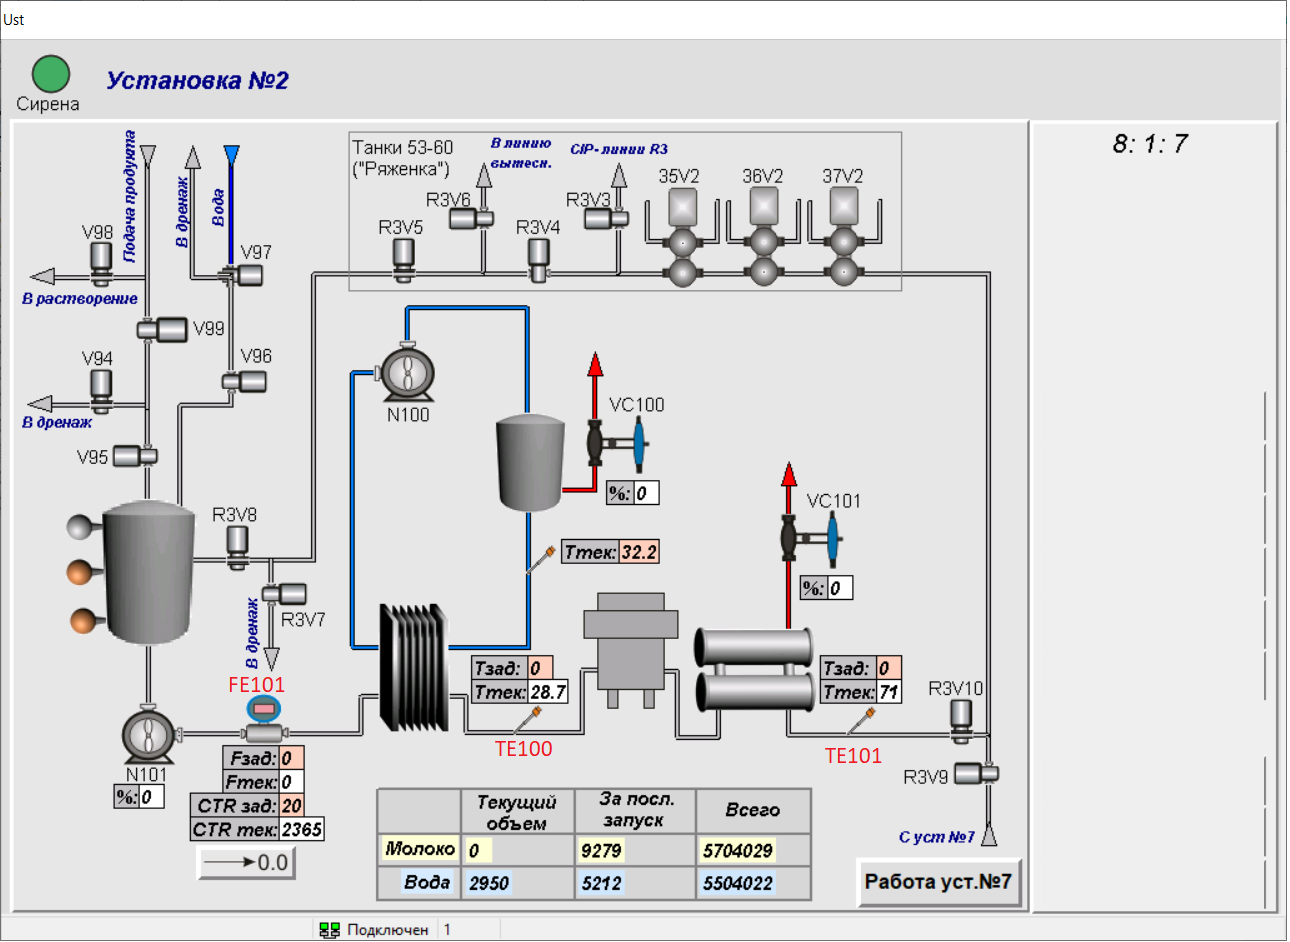
\includegraphics[width=\textwidth]{images/paster.png}
    \caption{\bfseries Рис 3.1: Схема пастеризационной установки на предприятии ОАО "Савушкин продукт"}
    \label{fig:NNBlackBox}
  \end{figure}

  \par \redline Давайте взглянем на данные с точки зрения инженерии машинного обучения и определим некоторые характеристики данных. 

  \par \redline Для начала определим, достаточно ли данных для обучения. Имеется 7 файлов формата .csv, которые хранят информацию о технологическом процессе пастеризационной установки в течении 70995465 секунд или около 835.5 дней. За такой промежуток времени мы имеем 20123304 данный различных сидов. Поэтому можно с уверенностью сказать, что данных для проекта машинного обучения достаточно, а потому способны обеспечить достаточную обобщающую способность модели.

  \par \redline Данные описывают состояние пастеризационной установки круглые сутки в течении почти двух с половиной лет. Это нам позволяет говорить о большом покрытии данных. Это значит, что данные отражают все состояния объекта. Также мы можем говорить об информативности данных, поскольку оно отражают реальный технологический процесс.

  \par \redline Для прояснения дальнейших моментов, хочется в очередной раз обратить внимание на то, что данные были собраны с помощью датчиков, поэтому данные являются надёжными и не подверженными к большинству видов смещений – несогласованность данных с явлением, которые эти данные описывают.  Однако, эти данные всё-таки могут быть подвержены систематическому смещению, возникающее при измерениях или наблюдениях с помощью некоторого устройства, поскольку качество и характеристики устройства влияют на качество самих данных. Однако, мы может игнорировать данное смещение, поскольку дальнейшая работа будет построена с теми же датчиками, а потому мы может говорить и о ещё одной черте качественных данных, а именно о том, что данные отражают реальный входы. Это значит, что будущая сеть будет обучаться на данных, представленных в таком виде, в котором они будут в последствии приходить на входы сети. В будущем мы ещё упомянем это свойство и расскажем о некоторых подводных камнях, связанные с этим.

  \par \redline Также хочется отметить, что данные не являются результатом обратной связи, т.е. не являются результатом самой модели, поскольку при сборе данных модели ещё не существовало.

  \par \redline Для дальнейшего описания данных необходимо их визуализировать.

  \begin{figure}
    \centering
    \def\svgwidth{\textwidth}
    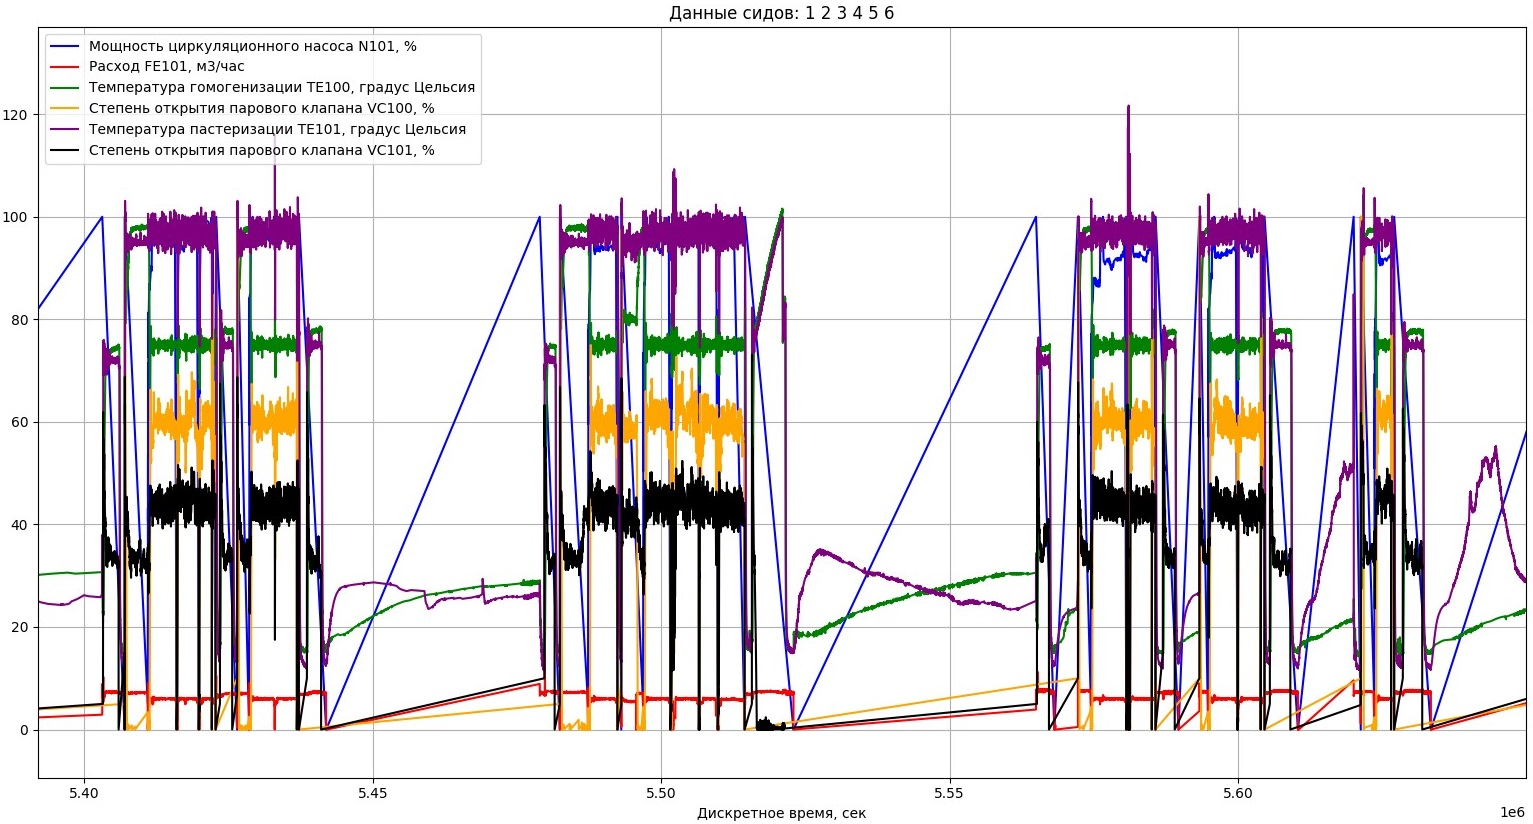
\includegraphics[width=\textwidth]{images/data_1_visual.jpg}
    \caption{\bfseries Рис 3.2: Визуализация данный 1-ого файла.}
    \label{fig:NNBlackBox}
  \end{figure}

  \begin{figure}
    \centering
    \def\svgwidth{\textwidth}
    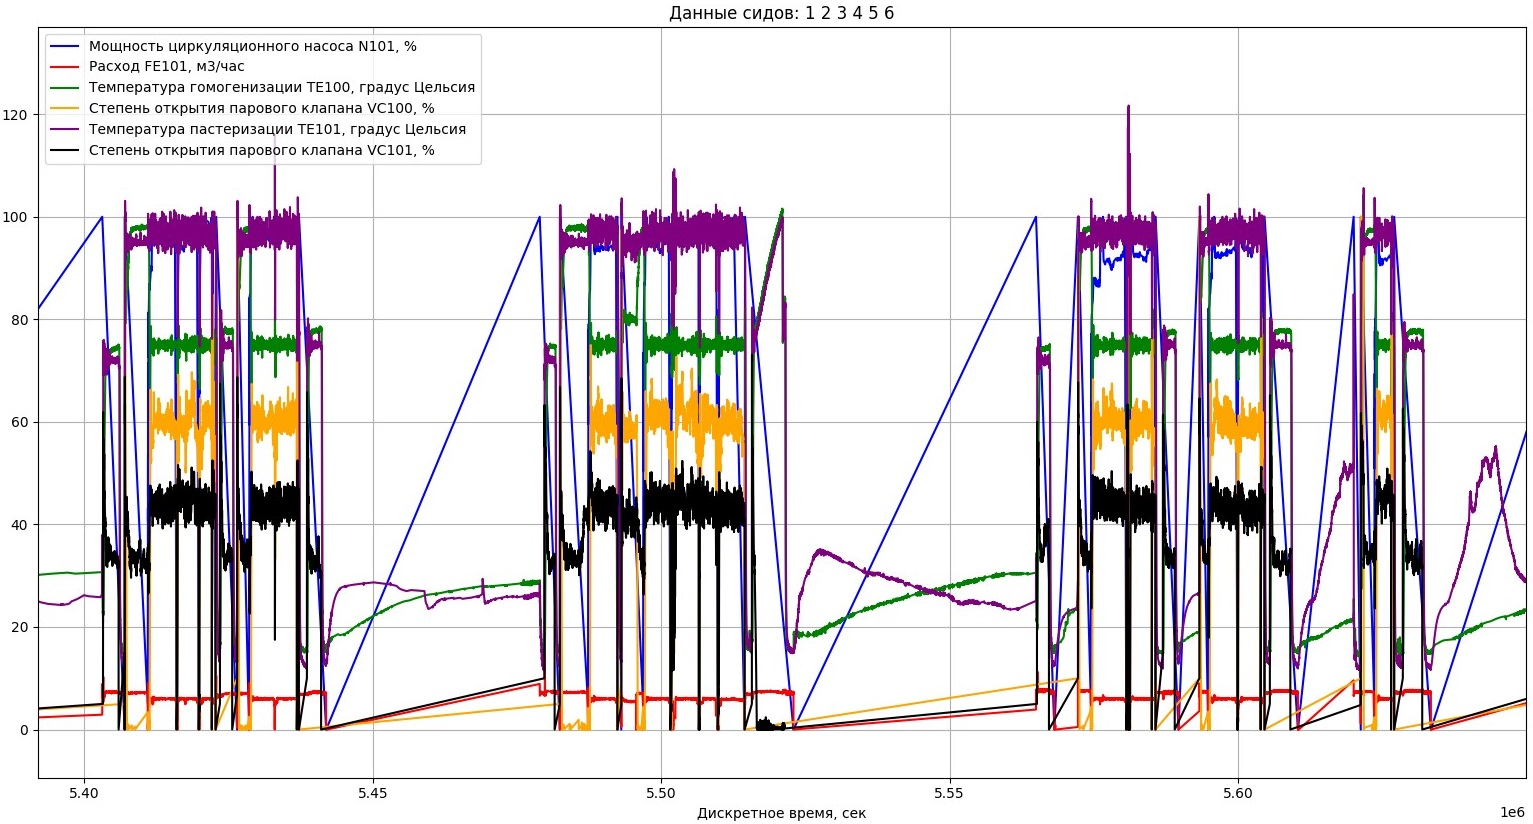
\includegraphics[width=\textwidth]{images/data_1_visual.jpg}
    \caption{\bfseries Рис 3.3: Визуализация данный 2-ого файла с растяжением масштаба по оси абсцисс.}
    \label{fig:NNBlackBox}
  \end{figure}

  \begin{figure}
    \centering
    \def\svgwidth{\textwidth}
    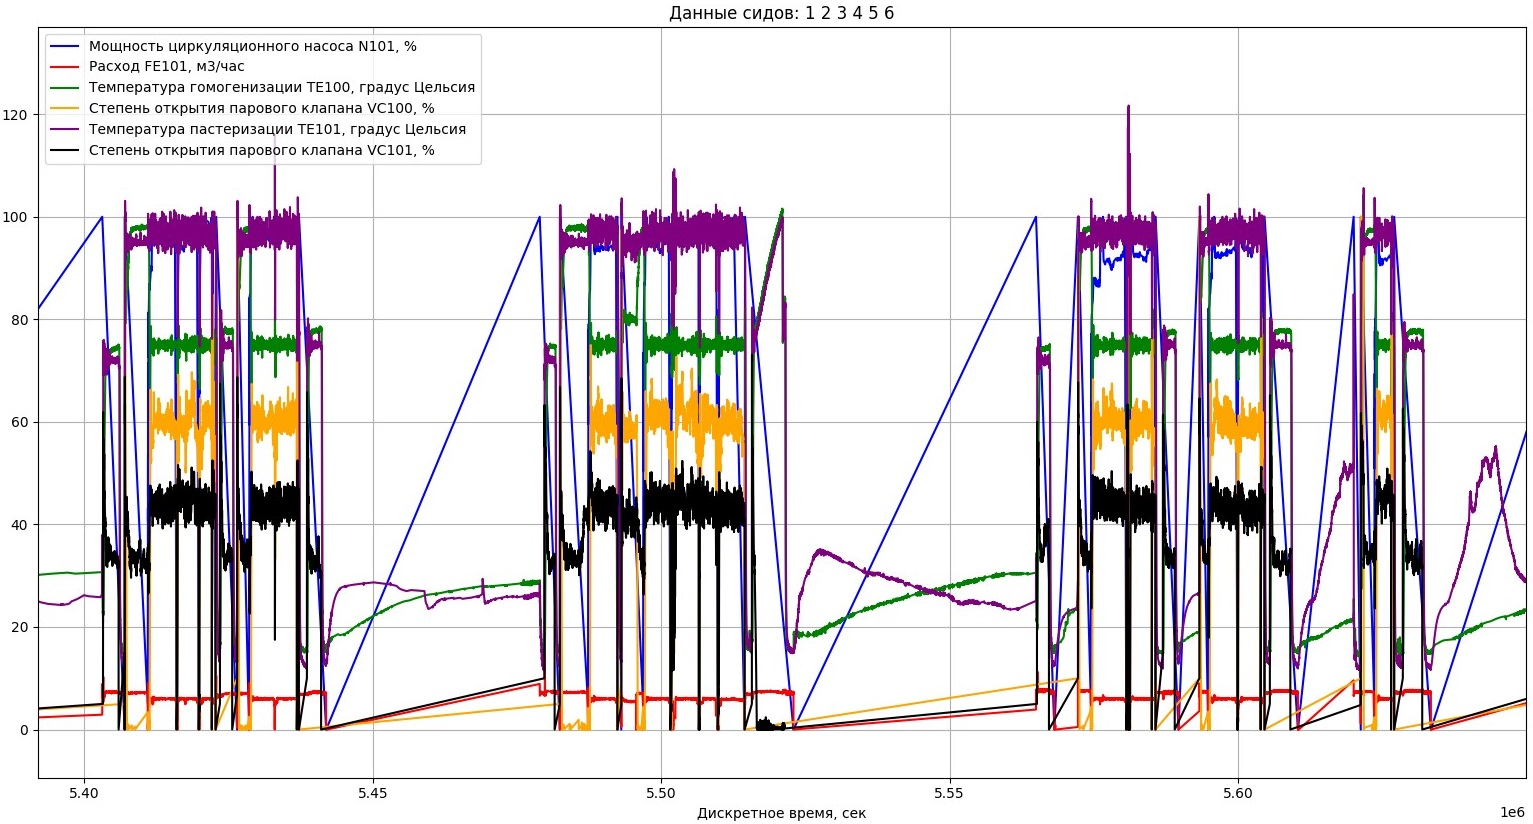
\includegraphics[width=\textwidth]{images/data_1_visual.jpg}
    \caption{\bfseries Рис 3.4: Визуализация данный 3-ого файла с cуженным масштаба по оси абсцисс.}
    \label{fig:NNBlackBox}
  \end{figure}

  \par \redline Сравнивая данные на рисунках Рис…, хотелось бы пояснить, что данные остальных файлов очень похожи с данными на Рис…. Из этого делаем вывод, что данные на Рис… содержат аномалии, поскольку схожее поведение пастеризационной установки средствами визуализации в других файлах выявлено не было. Это значит, что мы имеем большинство данных без аномалий, но также имеем и примеры данных с аномалиями. 

  \par \redline Продолжим изучение данных.

  ИНФОГРАФИКА
}

\titlespace
\subsection*{ 
  \cyrillicfont 
  \fontsize{14pt}{0pt}\selectfont
  \englishfont
  \redline
  3.1 Обработка данных и их подготовка к прогнозированию
} 
\titlespace

{\cyrillicfont 
\fontsize{13pt}{16.25pt}\selectfont 
\englishfont 

  \par \redline И так, пришло время поговорить об обработке данных. Она нужна в основном для того, чтобы сделать данные понятными для модели, а также для заполнения «дыр» в данных или для различного рода аппроксимаций. Под «дырами» понимаются некоторые пропущенные значения, например, определено время и значение датчика, а сид пропущен, вместо него пустое поле. Также под «дырами» понимаются магические числа, вроде -1, 99999 и другие, говорящие о том, что значение, заменённое магическим числом, неизвестно, но пустого поля быть не может. В данных формата ocdf такой проблемы не наблюдается, однако не стоит об этом забывать. В бедующем мы ещё с этим столкнёмся.

  \par \redline Поговорим о хранении данных. Начальные данные хранятся в файлах формата .csv. Это весьма распространённый формат файлов для хранения данных, представленных в форме временных рядов. В них данные хранятся в следующем виде: <сид>;<время>;<значение>. В дальнейшем такой вид данных мы будем обозначать как ocdf-формат данных. Преимуществом хранения данных в таких файлах является их доступность для любых программ или языков. Однако такие файлы занимают большой объём, а также при работе с такими файлами чтение или запись информации занимает большое количество времени.  

  \par \redline Для решения основных проблем при работе с файлами формата .csv, было принято решение использовать бинарные файлы формата .bin для хранения данных. Это дало возможность уменьшить занимаемый объём файлов, но самое главное, это позволило значительно сократить время для записи или чтения информации. Для примера: тут будут примеры.   Разница чтения данных составляет , а разница записи данных составляет .

  \par \redline В ходе работы с моделью возможно не будет необходимости работать со всеми сидами, а только с определёнными. Для того, чтобы не задействовать оперативную память зря, необходимо разделить данные по сидам.   

  \par \redline Для формирования различных наборов данных необходима возможность обрезать данные до необходимого нам диапазона или количества. Для более полного понимая смысла обрезки данных в очередной раз обратимся к инженерии машинного обучения: весь набор данных делится на обучающий, контрольный и тестовый наборы. Обучающий набор используется для непосредственного обучения модели. На контрольном наборе проверяется качество модели и подбираются её параметры, другими словами, настраивается модель. На тестовом наборе проверяется работа сети и делается вердикт о готовности модели. 

  \par \redline Для формирования различных наборов данных как раз и нужны различные способы обрезки данных, позволяющие отбросить данные как справа, так и слева. 
 
  \par \redline Также необходима возможность добавлять новые данные, чтобы при обучении сеть, которая учитывает зависимости между различными датчиками, была обеспечена данными необходимых сидов.  

  \par \redline Учитывая особенности вида данных, которые поуступают на предиктовый детектор системы Kaspersky MLAD, а также ввиду того, что данная модель будет работать в режиме реального времени и данные будут поступать через некоторый промежуток времени, то необходимо сделать так, чтобы начальные данные также были равноудалены друг от друга относительно оси времени. Однако, взаимное удаление точек по оси времени в начальных данные не постоянно. Эти диапазоны необходимо выровнять, чтобы повысить схожесть реальных входов и входов при обучении модели. Другими словами, необходимо преобразовать начальный данные в такие данные, в которых каждое значение времени представляло собой арифметическую прогрессию:

  \[t_i = t_0 + i \times r\]

  где $t_0$ {--} начальное значение времени; $r$ {--} необходимое расстояние между точками, представляющее собой некоторую константу, которую может задать пользователь; $i$ 
  {--} номер точки, итерации, элемента прогрессии; $t_i$ {--} i-ыт элемент прогрессии. 

  \par \redline Теперь осталось определить значение ординаты для каждого рассчитанного значения времени. Для этого было принято решение воспользоваться аналитической геометрией и взять за основу уравнение прямой, проходящей через две точки.  

  \[\frac{x - x_1}{x_2 - x_1} = \frac{y - y_1}{y_2 - y_1}\]

  где, точка $\left(х, у\right)$ – это точка, которую необходимо найти между точками $\left(х_1, у_1\right)$ и $\left(х_2, у_2\right)$, взятых из реальных данных. При этом, известно, что $х_1 \leq x \leq x_2$. 

  \par \redline Для определение ординаты для i-того элемента прогресии необходимо взять две ближайших точки из реальных данных относительно оси абсцисс к искомой точке. Тогда получим выражение для определение ординаты:

  \[y = \left(\frac{\left(x - x_1\right) \times \left(y_2 - y_1\right)}{x_2 - x_1}\right) + y_1\]

  \par \redline Таким образом можно получить аппроксимированные данные, где взаимное удаление между двумя соседними точками будет везде постоянным.  

  \par \redline Благодаря возможности выравнивания диапазонов по оси абсцисс, появляется возможность создать, так называемые, аккуратные данные – данные представленные в виде упорядоченной таблицы без каких-либо «дыр». Однако, если попытаться перевести имеющиеся данные в табличный формат, который в последствии мы будем называть tdf форматом, то мы обнаружим, что начальные данные содержат информацию о значениях датчика при неповторяющихся уникальных значениях времени. Это значит, что если для некоторого датчика определено его значение в некоторый момент времени в начальных данных, то значение другие датчиков в этот же момент времени не известно. Для решения данной проблемы нам помогут операции парсинга и выравнивания диапазонов по оси абсцисс. Чтобы преобразовать данные формата ocdf в данные формата tdf необходимо выполнить несколько последовательных действий. 

  \par \redline Для начала необходимо убедиться, что данные формата ocdf содержат в себе данные всех сидов, а после распарсить данные по сидам. Затем обрезать все последовательности распарсенных данных с их начала и до максимального значения времени первых элементов последовательности распарсенных данных, также с минимального значения времени последних элементов последователи распарсенных данных до конца всех последовательностей распарсенных данных. Если в обрезаемой последовательности нет точки с граничным значением времени, тогда необходимо найти эту точку средствами уравнения прямой через две точки, описанной выше. Далее выровнять диапазоны по оси абсцисс для всех расперсенных данных. В заключении требуется соединить полученные данные в одну последовательность следующего вида. Формат tdf выглядит следующим образом:

  \par <время>;<ЗД1>;< ЗД2>;< ЗД3>;< ЗД4>;< ЗД5>;< ЗД6>

  где, ЗДН – значение датчика под номером Н. 

  \par \redline Выполнив алгоритм, мы получаем аккуратные данные в табличном виде. Хранить их предпочтительно в бинарном виде, поскольку в формате .csv такие данные будут занимать очень много места, да и время на их чтение или запись будет довольно-таки немаленьким. 

  \par \redline Учитывая некоторые особенности активирующих функций, некоторые модели будут содержать в себе встроенные модули преобразования данных из одного диапазона по оси ординат в эквивалентные данные из другого диапазона по оси ординат и наоборот, сохраняя значения по оси абсцисс. Такую операцию мы будет в дальнейшем называть скейлингом.

  \par \redline Данная задача выглядит следующим образом: пусть есть $y \in \left[a; b\right]$, а необходимо преобразовать $y$ в эквивалентное значение $z \in \left[c; d\right]$. Тогда для операции скейлинга имеем следующее выражение:

  \[z = \frac{\left(y - a\right) \times \left(b - a\right)}{d - c} + c\]

  \par \redline А для того, чтобы восстановить эти значения, т.е. провести операцию обратного скейлинга, необходимо использовать следующее выражение: 

  \[y = \frac{\left(z - c\right) \times \left(d - c\right)}{b - a} + a\]

  \par \redline Операции скейлинга предполагают те модели, выходные элементы которых используют активирующие функции, имеющие горизонтальные асимптоты. Другими словами, активирующие функции, ограниченные по оси ординат. В таком случае, перед обучение или прогнозированием данных, будет проведена операция скейлинга, после основная операция, а в завершении операция обратного скейлинга. Т.к. данные уже изучены, можно с полной уверенность сказать, что операцию скейлинга для данных по оси ординат мы можем провести. 

  \par
}

